% https://tex.stackexchange.com/questions/452323/tikz-nested-block-diagram-with-boxed-text-inside-other-blocks
\documentclass[border=3.14mm,tikz]{standalone}
\usepackage{tikz}

\usetikzlibrary{calc}
\usetikzlibrary{shapes.arrows}
\usetikzlibrary{positioning,fit,backgrounds}

\begin{document}
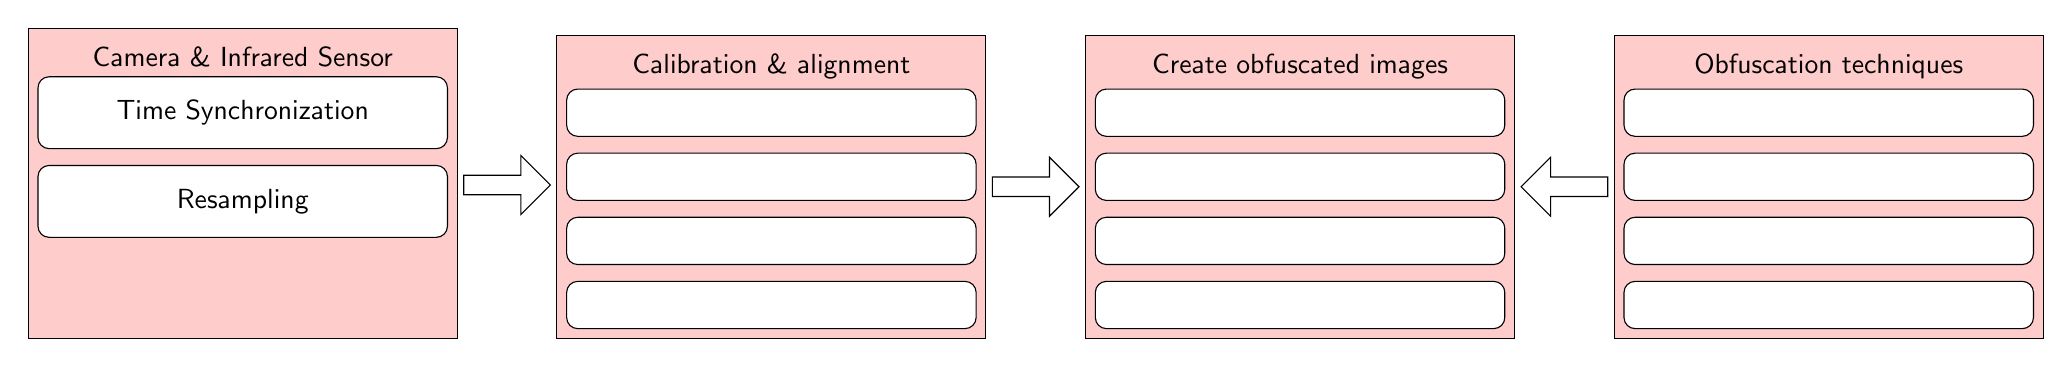
\begin{tikzpicture}[mynode/.style = {rectangle, draw, align=center,
            text width=4cm,fill=white,
            inner xsep=6mm, inner ysep=3mm, rounded corners},
            my arrow/.style={single arrow, draw,minimum height=1.1cm},
rotate border/.style={shape border uses incircle, shape border rotate=#1},
            font=\sffamily]
    \node[mynode, label={[name=lab]Camera \& Infrared Sensor}] (inner1) {Time Synchronization};
    \node[mynode, below=2mm of inner1] (justbelow1) {Resampling};
    %
    \node[right=1.5cm of inner1, mynode, label={[name=cal]Calibration \& alignment}] (inner2) {};
    \node[mynode, below=2mm of inner2] (justbelow2) {};
    \node[mynode, below=2mm of justbelow2] (justbelow2b) {};
    \node[mynode, below=2mm of justbelow2b] (justbelow2c) {};
    %
    \node[right=1.5cm of inner2, mynode, label={[name=img]Create obfuscated
    images}] (inner3) {};
    \node[mynode, below=2mm of inner3] (justbelow3) {};
    \node[mynode, below=2mm of justbelow3] (justbelow3b) {};
    \node[mynode, below=2mm of justbelow3b] (justbelow3c) {};
    %
    \node[right=1.5cm of inner3, mynode, label={[name=tech]Obfuscation
    techniques}] (inner4) {};
    \node[mynode, below=2mm of inner4] (justbelow4) {};
    \node[mynode, below=2mm of justbelow4] (justbelow4b) {};
    \node[mynode, below=2mm of justbelow4b] (justbelow4c) {};
    \begin{scope}[on background layer]
    \node[fit={(lab) (inner1) (justbelow4c.south-|inner1.south)}, draw,fill=red!20] (outer1) {};
    \node[fit={(cal) (inner2) (justbelow2c)}, draw,fill=red!20] (outer2) {};
    \node[fit={(img) (inner3) (justbelow3c)}, draw,fill=red!20] (outer3) {};
    \node[fit={(tech) (inner4) (justbelow4c)}, draw,fill=red!20] (outer4) {};
    \end{scope}
    \path (outer1) -- (outer2) node[pos=0.45,my arrow]{}
    (outer2) -- (outer3) node[pos=0.45,my arrow]{}
    (outer4) -- (outer3) node[pos=0.45,my arrow,shape border rotate=180]{};
    \end{tikzpicture}
\end{document}